%%% MATH110-PS033-Solutions.tex --- 
%% 
%% Filename: MATH110-PS033-Solutions.tex
%% Description: 
%% Author: U-ORONYA\edwar
%% Maintainer: 
%% Created: Sun Jan 29 09:55:51 2023 (-0600)
%% Version: 
%% Package-Requires: ()
%% Last-Updated: Sun Jan 29 10:08:13 2023 (-0600)
%%           By: U-ORONYA\edwar
%%     Update #: 3
%% URL: 
%% Doc URL: 
%% Keywords: 
%% Compatibility: 
%% 
%%%%%%%%%%%%%%%%%%%%%%%%%%%%%%%%%%%%%%%%%%%%%%%%%%%%%%%%%%%%%%%%%%%%%%
%% 
%%% Commentary: 
%% 
%% 
%% 
%%%%%%%%%%%%%%%%%%%%%%%%%%%%%%%%%%%%%%%%%%%%%%%%%%%%%%%%%%%%%%%%%%%%%%
%% 
%%% Change Log:
%% 
%% 
%%%%%%%%%%%%%%%%%%%%%%%%%%%%%%%%%%%%%%%%%%%%%%%%%%%%%%%%%%%%%%%%%%%%%%
%%
%% Copyright (C) 2023 Edward Doolittle 
%% 
%%%%%%%%%%%%%%%%%%%%%%%%%%%%%%%%%%%%%%%%%%%%%%%%%%%%%%%%%%%%%%%%%%%%%%
%% 
%%% Code:


\documentclass{article}
\usepackage{amsmath}
\usepackage{fullpage}
%\usepackage{graphicx}
\usepackage[aux]{rerunfilecheck}
\usepackage{tikz}
\usetikzlibrary{calc}
%\usepackage{pgfmath}

\newcommand{\ds}{\displaystyle}

% Macros for MATH 110 course dates

\newcommand{\commonTheme}{metropolis}
\newcommand{\commonColorTheme}{metropolis}

\newcommand{\commonAuthor}{Edward Doolittle}
\newcommand{\commonInstitute}{Department of Indigenous Knowledge and
  Science \\ First Nations University of Canada}
\newcommand{\commonCourse}{MATH 110 Calculus I}
\newcommand{\commonTerm}{202510}
\newcommand{\commonDate}{January 6, 2025}

% Review Material

% Lab 0
\newcommand{\commonEventNegativeOne}{LabNegativeOne}
\newcommand{\commonDateLabNegativeOne}{Monday, January 6, 2025}
\newcommand{\commonTitleLabNegativeOne}{MATH 110 Lab 0}
\newcommand{\commonSubtitleLabNegativeOne}{No Lab; Course Opens}

% Section 001
\newcommand{\commonEventZeroZeroOne}{ZeroZeroOne}
\newcommand{\commonDateZeroZeroOne}{Tuesday, January 7, 2025}
\newcommand{\commonTitleZeroZeroOne}{MATH 110 Review 0.1}
\newcommand{\commonSubtitleZeroZeroOne}{Review of Algebra}
\newcommand{\commonPSTitleZeroZeroOne}{MATH 110 Review Problem Set 0.1}

% Section 00A
\newcommand{\commonEventZeroZeroA}{ZeroZeroA}
\newcommand{\commonDateZeroZeroA}{Tuesday, January 7, 2025}
\newcommand{\commonTitleZeroZeroA}{MATH 110 Review 0.A}
\newcommand{\commonSubtitleZeroZeroA}{Review of Inequalities and
  Absolute Values}
\newcommand{\commonPSTitleZeroZeroA}{MATH 110 Review Problem Set 0.A}

% Section 00B
\newcommand{\commonEventZeroZeroB}{ZeroZeroB}
\newcommand{\commonDateZeroZeroB}{Tuesday, January 7, 2025}
\newcommand{\commonTitleZeroZeroB}{MATH 110 Review 0.B}
\newcommand{\commonSubtitleZeroZeroB}{Review of Coordinate Geometry
  and Lines}
\newcommand{\commonPSTitleZeroZeroB}{MATH 110 Review Problem Set 0.B}

% Section 00C
\newcommand{\commonEventZeroZeroC}{ZeroZeroC}
\newcommand{\commonDateZeroZeroC}{Thursday, January 9, 2025}
\newcommand{\commonTitleZeroZeroC}{MATH 110 Review 0.C}
\newcommand{\commonSubtitleZeroZeroC}{Review of Graphs of Second
  Degree Equations}
\newcommand{\commonPSTitleZeroZeroC}{MATH 110 Review Problem Set 0.C}

% Section 00D
\newcommand{\commonEventZeroZeroD}{ZeroZeroD}
\newcommand{\commonDateZeroZeroD}{Thursday, January 9, 2025}
\newcommand{\commonTitleZeroZeroD}{MATH 110 Review 0.D}
\newcommand{\commonSubtitleZeroZeroD}{Review of Trigonometry}
\newcommand{\commonPSTitleZeroZeroD}{MATH 110 Review Problem Set 0.D}

% Section 011
\newcommand{\commonEventZeroOneOne}{ZeroOneOne}
\newcommand{\commonDateZeroOneOne}{Thursday, January 9, 2025}
\newcommand{\commonTitleZeroOneOne}{MATH 110 Review 1.1}
\newcommand{\commonSubtitleZeroOneOne}{Review of Functions}
\newcommand{\commonPSTitleZeroOneOne}{MATH 110 Review Problem Set 1.1}


% Main Course

% Lab 1
\newcommand{\commonEventZero}{LabZero}
\newcommand{\commonDateLabZero}{Monday, January 13, 2025}
\newcommand{\commonTitleLabZero}{MATH 110 Lab 1}
\newcommand{\commonSubtitleLabZero}{Quiz 0: STACK, Onboarding}

% Section 1.4
\newcommand{\commonEventOne}{ZeroOneFour}
\newcommand{\commonDateZeroOneFour}{Tuesday, January 14, 2025}
\newcommand{\commonTitleZeroOneFour}{MATH 110 Lecture 1.4}
\newcommand{\commonSubtitleZeroOneFour}{The Tangent and Velocity Problems}
\newcommand{\commonPSTitleZeroOneFour}{MATH 110 Problem Set 1.4}

% Section 1.5
\newcommand{\commonEventTwo}{ZeroOneFive}
\newcommand{\commonDateZeroOneFive}{Thursday, January 16, 2025}
\newcommand{\commonTitleZeroOneFive}{MATH 110 Lecture 1.5}
\newcommand{\commonSubtitleZeroOneFive}{The Limit of a Function}
\newcommand{\commonPSTitleZeroOneFive}{MATH 110 Problem Set 1.5}

% Lab 2
\newcommand{\commonEventThree}{LabOne}
\newcommand{\commonDateLabOne}{Monday, January 20, 2025}
\newcommand{\commonTitleLabOne}{MATH 110 Lab 2}
\newcommand{\commonSubtitleLabOne}{Quiz 1: Review}

% Section 1.6
\newcommand{\commonEventFour}{ZeroOneSix}
\newcommand{\commonDateZeroOneSix}{Tuesday, January 21, 2025}
\newcommand{\commonTitleZeroOneSix}{MATH 110 Lecture 1.6}
\newcommand{\commonSubtitleZeroOneSix}{Calculating Limits Using the Limit Laws}
\newcommand{\commonPSTitleZeroOneSix}{MATH 110 Problem Set 1.6}

% Section 1.7
\newcommand{\commonEventFive}{ZeroOneSeven}
\newcommand{\commonDateZeroOneSeven}{(Not covered)}
\newcommand{\commonTitleZeroOneSeven}{MATH 110 Lecture 1.7}
\newcommand{\commonSubtitleZeroOneSeven}{The Precise Definition of a Limit}
\newcommand{\commonPSTitleZeroOneSeven}{MATH 110 Problem Set 1.7}

% Section 1.8
\newcommand{\commonEventSix}{ZeroOneEight}
\newcommand{\commonDateZeroOneEight}{Thursday, January 23, 2025}
\newcommand{\commonTitleZeroOneEight}{MATH 110 Lecture 1.8}
\newcommand{\commonSubtitleZeroOneEight}{Continuity}
\newcommand{\commonPSTitleZeroOneEight}{MATH 110 Problem Set 1.8}

% Lab 3
\newcommand{\commonEventSeven}{LabTwo}
\newcommand{\commonDateLabTwo}{Monday, January 27, 2025}
\newcommand{\commonTitleLabTwo}{MATH 110 Lab 3}
\newcommand{\commonSubtitleLabTwo}{Quiz 2: Sections 1.4, 1.5}

% Section 2.1
\newcommand{\commonEventEight}{ZeroTwoOne}
\newcommand{\commonDateZeroTwoOne}{Tuesday, January 28, 2025}
\newcommand{\commonTitleZeroTwoOne}{MATH 110 Lecture 2.1}
\newcommand{\commonSubtitleZeroTwoOne}{Derivatives and Rates of Change}
\newcommand{\commonPSTitleZeroTwoOne}{MATH 110 Problem Set 2.1}

% Section 2.2
\newcommand{\commonEventNine}{ZeroTwoTwo}
\newcommand{\commonDateZeroTwoTwo}{Thursday, January 30, 2025}
\newcommand{\commonTitleZeroTwoTwo}{MATH 110 Lecture 2.2}
\newcommand{\commonSubtitleZeroTwoTwo}{The Derivative as a Function}
\newcommand{\commonPSTitleZeroTwoTwo}{MATH 110 Problem Set 2.2}

% Lab 4
\newcommand{\commonEventTen}{LabThree}
\newcommand{\commonDateMTOne}{Monday, February 3, 2025} 
\newcommand{\commonDateLabThree}{Monday, February 3, 2025}
\newcommand{\commonTitleLabThree}{MATH 110 Lab 4}
\newcommand{\commonSubtitleLabThree}{Midterm: Review, Chapter 1}

% Section 2.3
\newcommand{\commonEventEleven}{ZeroTwoThree}
\newcommand{\commonDateZeroTwoThree}{Tuesday, February 4, 2025}
\newcommand{\commonTitleZeroTwoThree}{MATH 110 Lecture 2.3}
\newcommand{\commonSubtitleZeroTwoThree}{Differentiation Formulas}
\newcommand{\commonPSTitleZeroTwoThree}{MATH 110 Problem Set 2.3}

% Section 2.4
\newcommand{\commonEventTwelve}{ZeroTwoFour}
\newcommand{\commonDateZeroTwoFour}{Thursday, February 6, 2025}
\newcommand{\commonTitleZeroTwoFour}{MATH 110 Lecture 2.4}
\newcommand{\commonSubtitleZeroTwoFour}{Derivatives of Trigonometric Functions}
\newcommand{\commonPSTitleZeroTwoFour}{MATH 110 Problem Set 2.4}

% Lab 5
\newcommand{\commonEventThirteen}{LabFour}
\newcommand{\commonDateLabFour}{Monday, February 10, 2025}
\newcommand{\commonTitleLabFour}{MATH 110 Lab 5}
\newcommand{\commonSubtitleLabFour}{Quiz 3: Sections 2.1, 2.2}

% Section 2.5
\newcommand{\commonEventFourteen}{ZeroTwoFive}
\newcommand{\commonDateZeroTwoFive}{Tuesday, February 11, 2025}
\newcommand{\commonTitleZeroTwoFive}{MATH 110 Lecture 2.5}
\newcommand{\commonSubtitleZeroTwoFive}{The Chain Rule}
\newcommand{\commonPSTitleZeroTwoFive}{MATH 110 Problem Set 2.5}

% Section 2.6
\newcommand{\commonEventFifteen}{ZeroTwoSix}
\newcommand{\commonDateZeroTwoSix}{Thursday, February 13, 2025}
\newcommand{\commonTitleZeroTwoSix}{MATH 110 Lecture 2.6}
\newcommand{\commonSubtitleZeroTwoSix}{Implicit Differentiation}
\newcommand{\commonPSTitleZeroTwoSix}{MATH 110 Problem Set 2.6}

% Lab 6
\newcommand{\commonEventSixteen}{LabFive}
\newcommand{\commonDateLabFive}{Monday, February 24, 2025}
\newcommand{\commonTitleLabFive}{MATH 110 Lab 6}
\newcommand{\commonSubtitleLabFive}{Quiz 4: Sections 2.3, 2.4}

% Section 2.7
\newcommand{\commonEventSeventeen}{ZeroTwoSeven}
\newcommand{\commonDateZeroTwoSeven}{Tuesday, February 25, 2025}
\newcommand{\commonTitleZeroTwoSeven}{MATH 110 Lecture 2.7}
\newcommand{\commonSubtitleZeroTwoSeven}{Rates of Change in the
  Natural and Social Sciences}
\newcommand{\commonPSTitleZeroTwoSeven}{MATH 110 Problem Set 2.7}

% Section 2.8
\newcommand{\commonEventEighteen}{ZeroTwoEight}
\newcommand{\commonDateZeroTwoEight}{Thursday, February 27, 2025}
\newcommand{\commonTitleZeroTwoEight}{MATH 110 Lecture 2.8}
\newcommand{\commonSubtitleZeroTwoEight}{Related Rates}
\newcommand{\commonPSTitleZeroTwoEight}{MATH 110 Problem Set 2.8}

% Lab 7
\newcommand{\commonEventNineteen}{LabSix}
\newcommand{\commonDateLabSix}{Monday, March 3, 2025}
\newcommand{\commonTitleLabSix}{MATH 110 Lab 7}
\newcommand{\commonSubtitleLabSix}{Quiz 5: Sections 2.5, 2.6}

% Section 3.1
\newcommand{\commonEventTwenty}{ZeroThreeOne}
\newcommand{\commonDateZeroThreeOne}{Tuesday, March 4, 2025}
\newcommand{\commonTitleZeroThreeOne}{MATH 110 Lecture 3.1}
\newcommand{\commonSubtitleZeroThreeOne}{Maximum and Minimum Values}
\newcommand{\commonPSTitleZeroThreeOne}{MATH 11 Problem Set 3.1}

% Section 3.2
\newcommand{\commonEventTwentyOne}{ZeroThreeTwo}
\newcommand{\commonDateZeroThreeTwo}{Thursday, March 6, 2025}
\newcommand{\commonTitleZeroThreeTwo}{MATH 110 Lecture 3.2}
\newcommand{\commonSubtitleZeroThreeTwo}{The Mean Value Theorem}
\newcommand{\commonPSTitleZeroThreeTwo}{MATH 110 Problem Set 3.2}

% Lab 8
\newcommand{\commonEventTwentyTwo}{LabSeven}
\newcommand{\commonDateMTTwo}{Monday, March 10, 2025}
\newcommand{\commonDateLabSeven}{Monday, March 10, 2025}
\newcommand{\commonTitleLabSeven}{MATH 110 Lab 8}
\newcommand{\commonSubtitleLabSeven}{Midterm: Chapter 2}

% Section 3.3
\newcommand{\commonEventTwentyThree}{ZeroThreeThree}
\newcommand{\commonDateZeroThreeThree}{Tuesday, March 11, 2025}
\newcommand{\commonTitleZeroThreeThree}{MATH 110 Lecture 3.3}
\newcommand{\commonSubtitleZeroThreeThree}{How Derivatives Affect the
  Shape of a Graph}
\newcommand{\commonPSTitleZeroThreeThree}{MATH 110 Problem Set 3.3}

% Section 3.4
\newcommand{\commonEventTwentyFour}{ZeroThreeFour}
\newcommand{\commonDateZeroThreeFour}{Thursday, March 13, 2025}
\newcommand{\commonTitleZeroThreeFour}{MATH 110 Lecture 3.4}
\newcommand{\commonSubtitleZeroThreeFour}{Limits at Infinity;
  Horizontal Asymptotes}
\newcommand{\commonPSTitleZeroThreeFour}{MATH 110 Problem Set 3.4}

% Lab 9
\newcommand{\commonEventTwentyFive}{LabEight}
\newcommand{\commonDateLabEight}{Monday, March 17, 2025}
\newcommand{\commonTitleLabEight}{MATH 110 Lab 9}
\newcommand{\commonSubtitleLabEight}{Quiz 6: Sections 3.1, 3.2}

% Section 3.5
\newcommand{\commonEventTwentySix}{ZeroThreeFive}
\newcommand{\commonDateZeroThreeFive}{Tuesday, March 18, 2025}
\newcommand{\commonTitleZeroThreeFive}{MATH 110 Lecture 3.5}
\newcommand{\commonSubtitleZeroThreeFive}{Summary of Curve Sketching}
\newcommand{\commonPSTitleZeroThreeFive}{MATH 110 Problem Set 3.5}

% Section 3.7
\newcommand{\commonEventTwentySeven}{ZeroThreeSeven}
\newcommand{\commonDateZeroThreeSeven}{Thursday, March 20, 2025}
\newcommand{\commonTitleZeroThreeSeven}{MATH 110 Lecture 3.7}
\newcommand{\commonSubtitleZeroThreeSeven}{Optimization Problems}
\newcommand{\commonPSTitleZeroThreeSeven}{MATH 110 Problem Set 3.7}

% Lab 10
\newcommand{\commonEventTwentyEight}{LabNine}
\newcommand{\commonDateLabNine}{Monday, March 24, 2025}
\newcommand{\commonTitleLabNine}{MATH 110 Lab 10}
\newcommand{\commonSubtitleLabNine}{Quiz 7: Sections 3.3, 3.4}

% Section 4.1
\newcommand{\commonEventTwentyNine}{ZeroFourOne}
\newcommand{\commonDateZeroFourOne}{Tuesday, March 25, 2025}
\newcommand{\commonTitleZeroFourOne}{MATH 110 Lecture 4.1}
\newcommand{\commonSubtitleZeroFourOne}{Areas and Distances}
\newcommand{\commonPSTitleZeroFourOne}{MATH 110 Problem Set 4.1}

% Section 4.2
\newcommand{\commonEventThirty}{ZeroFourTwo}
\newcommand{\commonDateZeroFourTwo}{Thursday, March 27, 2025}
\newcommand{\commonTitleZeroFourTwo}{MATH 110 Lecture 4.2}
\newcommand{\commonSubtitleZeroFourTwo}{The Definite Integral}
\newcommand{\commonPSTitleZeroFourTwo}{MATH 110 Problem Set 4.2}

% Lab 11
\newcommand{\commonEventThirtyOne}{LabTen}
\newcommand{\commonDateLabTen}{Monday, March 31, 2025}
\newcommand{\commonTitleLabTen}{MATH 110 Lab 11}
\newcommand{\commonSubtitleLabTen}{Quiz 8: Sections 3.5, 3.7}

% Section 4.3
\newcommand{\commonEventThirtyTwo}{ZeroFourThree}
\newcommand{\commonDateZeroFourThree}{Tuesday, April 1, 2025}
\newcommand{\commonTitleZeroFourThree}{MATH 110 Lecture 4.3}
\newcommand{\commonSubtitleZeroFourThree}{The Fundamental Theorem of Calculus}
\newcommand{\commonPSTitleZeroFourThree}{MATH 110 Problem Set 4.3}

% Section 4.4
\newcommand{\commonEventThirtyThree}{ZeroFourFour}
\newcommand{\commonDateZeroFourFour}{Thursday, April 3, 2025}
\newcommand{\commonTitleZeroFourFour}{MATH 110 Lecture 4.4}
\newcommand{\commonSubtitleZeroFourFour}{Indefinite Integrals and the
  Net Change Theorem}
\newcommand{\commonPSTitleZeroFourFour}{MATH 110 Problem Set 4.4}

% Lab 12
\newcommand{\commonEventThirtyFour}{LabEleven}
\newcommand{\commonDateLabEleven}{Monday, April 7, 2025}
\newcommand{\commonTitleLabEleven}{MATH 110 Lab 12}
\newcommand{\commonSubtitleLabEleven}{Quiz 9: Sections 4.1, 4.2}

% Section 4.5
\newcommand{\commonEventThirtyFive}{ZeroFourFive}
\newcommand{\commonDateZeroFourFive}{Tuesday, April 8, 2025}
\newcommand{\commonTitleZeroFourFive}{MATH 110 Lecture 4.5}
\newcommand{\commonSubtitleZeroFourFive}{The Substitution Rule}
\newcommand{\commonPSTitleZeroFourFive}{MATH 110 Problem Set 4.5}

% Section 5.1
\newcommand{\commonEventThirtySix}{ZeroFiveOne}
\newcommand{\commonDateZeroFiveOne}{Thursday, April 10, 2025}
\newcommand{\commonTitleZeroFiveOne}{MATH 110 Lecture 5.1}
\newcommand{\commonSubtitleZeroFiveOne}{Areas Between Curves}
\newcommand{\commonPSTitleZeroFiveOne}{MATH 110 Problem Set 5.1}

% Lab 13
\newcommand{\commonEventThirtySeven}{LabTwelve}
\newcommand{\commonDateLabTwelve}{Monday, April 14, 2025}
\newcommand{\commonTitleLabTwelve}{MATH 110 Review Lab}
\newcommand{\commonSubtitleLabTwelve}{Bonus Quiz 10: Sections 4.3, 4.4}

% Final Class
\newcommand{\commonEventThirtyEight}{FinalClass}
\newcommand{\commonDateFinalClass}{Tuesday, April 15, 2025}
\newcommand{\commonTitleFinalClass}{MATH 110 Review Class}
\newcommand{\commonSubtitleFinalClass}{Answer Questions, Review for Exam}

% Final Exam
\newcommand{\commonEventThirtyNine}{Final}
\newcommand{\commonDateFinal}{Thursday, April 22, 2025}
\newcommand{\commonTitleFinal}{MATH 110 Final Exam}
\newcommand{\commonSubtitleFinal}{Comprehensive Exam: All Sections}

% Orphaned -- no longer part of the course

% Section 2.9
\newcommand{\commonDateZeroTwoNine}{Not part of the course}
\newcommand{\commonTitleZeroTwoNine}{MATH 110 Lecture 2.9}
\newcommand{\commonSubtitleZeroTwoNine}{Linear Approximations and Differentials}
\newcommand{\commonPSTitleZeroTwoNine}{MATH 110 Problem Set 2.9}


% % Introduction
% \newcommand{\commonEventOneDate}{Wednesday, September 8, 2010}
% \newcommand{\commonEventOneDesc}{Introduction to the Course}
% \newcommand{\commonDateZeroZeroZero}{September 8, 2010}
% \newcommand{\commonTitleZeroZeroZero}{MATH 104 Introduction}
% \newcommand{\commonSubtitleZeroZeroZero}{Outline of the Course}

% % Lecture 1
% \newcommand{\commonEventTwoDate}{Friday, September 10, 2010}
% \newcommand{\commonEventTwoDesc}{Lecture 1: Algebra}
% \newcommand{\commonDateZeroZeroOne}{September 10, 2010}
% \newcommand{\commonTitleZeroZeroOne}{MATH 104 Lecture 1}
% \newcommand{\commonSubtitleZeroZeroOne}{Review of Algebra}
% % associated evaluation ... factor this out?
% \newcommand{\commonPSTitleZeroZeroOne}{MATH 104 Problem Set 1}
% \newcommand{\commonEvalZeroZeroOne}{Quiz 1}
% \newcommand{\commonEvalDateZeroZeroOne}{Wednesday, September 15, 2010}

% % Lecture 2
% \newcommand{\commonEventThreeDate}{Monday, September 13, 2010}
% \newcommand{\commonEventThreeDesc}{Lecture 2: Appendix A}
% \newcommand{\commonDateZeroZeroA}{September 13, 2010}
% \newcommand{\commonTitleZeroZeroA}{MATH 104 Lecture 2}
% \newcommand{\commonSubtitleZeroZeroA}{Appendix A: Numbers, Inequalities, 
%   and Absolute Values}
% % associated evaluation ... factor this out?
% \newcommand{\commonPSTitleZeroZeroA}{MATH 104 Problem Set 2}
% \newcommand{\commonEvalZeroZeroA}{Quiz 2}
% \newcommand{\commonEvalDateZeroZeroA}{Wednesday, September 22, 2010}

% % Review 1
% \newcommand{\commonEventFourDate}{Wednesday, September 15, 2010}
% \newcommand{\commonEventFourDesc}{Review 1: Review Algebra; Quiz 1; Review Appendix A}
% \newcommand{\commonDateRZeroOne}{September 15, 2010}
% \newcommand{\commonTitleRZeroOne}{MATH 104 Review 1}
% \newcommand{\commonSubtitleRZeroOne}{Review of Algebra, Appendix A}

% % Lecture 3
% \newcommand{\commonEventFiveDate}{Friday, September 17, 2010}
% \newcommand{\commonEventFiveDesc}{Lecture 3: Appendix B}
% \newcommand{\commonDateZeroZeroB}{September 17, 2010}
% \newcommand{\commonTitleZeroZeroB}{MATH 104 Lecture 3}
% \newcommand{\commonSubtitleZeroZeroB}{Appendix B: Coordinate Geometry and Lines}
% % associated evaluation ... factor this out?
% \newcommand{\commonPSTitleZeroZeroB}{MATH 104 Problem Set 3}
% \newcommand{\commonEvalZeroZeroB}{Quiz 2}
% \newcommand{\commonEvalDateZeroZeroB}{Wednesday, September 22, 2010}

% % Lecture 4
% \newcommand{\commonEventSixDate}{Monday, Sepbember 20, 2010}
% \newcommand{\commonEventSixDesc}{Lecture 4: Appendix C}
% \newcommand{\commonDateZeroZeroC}{September 20, 2010}
% \newcommand{\commonTitleZeroZeroC}{MATH 104 Lecture 4}
% \newcommand{\commonSubtitleZeroZeroC}{Appendix C: Graphs of Second-Degree Equations}
% % associated evaluation ... factor this out?
% \newcommand{\commonPSTitleZeroZeroC}{MATH 104 Problem Set 4}
% \newcommand{\commonEvalZeroZeroC}{Midterm 0}
% \newcommand{\commonEvalDateZeroZeroC}{Wednesday, September 29, 2010}

% % Review 2
% \newcommand{\commonEventSevenDate}{Wednesday, September 22, 2010}
% \newcommand{\commonEventSevenDesc}{Review 2: Review Appendix B; Quiz 2; Review Appendix C}
% \newcommand{\commonDateRZeroTwo}{September 22, 2010}
% \newcommand{\commonTitleRZeroTwo}{MATH 104 Review 2}
% \newcommand{\commonSubtitleRZeroTwo}{Review of Appendices B and C}

% % Lecture 5
% \newcommand{\commonEventEightDate}{Friday, September 24, 2010}
% \newcommand{\commonEventEightDesc}{Lecture 5: Appendix D}
% \newcommand{\commonDateZeroZeroD}{September 24, 2010}
% \newcommand{\commonTitleZeroZeroD}{MATH 104 Lecture 5}
% \newcommand{\commonSubtitleZeroZeroD}{Appendix D: Trigonometry}
% % associated evaluation ... factor this out?
% \newcommand{\commonPSTitleZeroZeroD}{MATH 104 Problem Set 5}
% \newcommand{\commonEvalZeroZeroD}{Midterm 0}
% \newcommand{\commonEvalDateZeroZeroD}{Wednesday, September 29, 2010}

% % Lecture 6
% \newcommand{\commonEventNineDate}{Monday, September 27, 2010}
% \newcommand{\commonEventNineDesc}{Lecture 6: Section 1.1}
% \newcommand{\commonDateZeroOneOne}{September 27, 2010}
% \newcommand{\commonTitleZeroOneOne}{MATH 104 Lecture 6}
% \newcommand{\commonSubtitleZeroOneOne}{Section 1.1: Four Ways to Represent a Function}
% % associated evaluation ... factor this out?
% \newcommand{\commonPSTitleZeroOneOne}{MATH 104 Problem Set 6}
% \newcommand{\commonEvalZeroOneOne}{Quiz 3}
% \newcommand{\commonEvalDateZeroOneOne}{Wednesday, October 6, 2010}

% % Review 3
% \newcommand{\commonEventTenDate}{Wednesday, September 29, 2010}
% \newcommand{\commonEventTenDesc}{Review 3: Review Appendix D; 
%   Self-Assessment Midterm 0}
% \newcommand{\commonDateRZeroThree}{September 29, 2010}
% \newcommand{\commonTitleRZeroThree}{MATH 104 Review 3}
% \newcommand{\commonSubtitleRZeroThree}{Review of Appendix D}

% % Lecture 7
% \newcommand{\commonEventElevenDate}{Friday, October 1, 2010}
% \newcommand{\commonEventElevenDesc}{Lecture 7: Section 1.2}
% \newcommand{\commonDateZeroOneTwo}{October 1, 2010}
% \newcommand{\commonTitleZeroOneTwo}{MATH 104 Lecture 7}
% \newcommand{\commonSubtitleZeroOneTwo}{Section 1.2: Mathematical Models: A Catalog of Essential Functions}
% % associated evaluation ... factor this out?
% \newcommand{\commonPSTitleZeroOneTwo}{MATH 104 Problem Set 7}
% \newcommand{\commonEvalZeroOneTwo}{Quiz 3}
% \newcommand{\commonEvalDateZeroOneTwo}{Wednesday, October 6, 2010}

% % Lecture 8
% \newcommand{\commonEventTwelveDate}{Monday, October 4, 2010}
% \newcommand{\commonEventTwelveDesc}{Lecture 8: Section 1.3}
% \newcommand{\commonDateZeroOneThree}{October 4, 2010}
% \newcommand{\commonTitleZeroOneThree}{MATH 104 Lecture 8}
% \newcommand{\commonSubtitleZeroOneThree}{Section 1.3: New Functions from Old Functions}
% % associated evaluation ... factor this out?
% \newcommand{\commonPSTitleZeroOneThree}{MATH 104 Problem Set 8}
% \newcommand{\commonEvalZeroOneThree}{Quiz 4}
% \newcommand{\commonEvalDateZeroOneThree}{Wednesday, October 13, 2010}

% % Review 4
% \newcommand{\commonEventThirteenDate}{Wednesday, October 6, 2010}
% \newcommand{\commonEventThirteenDesc}{Review 4: Review 1.1, 1.2; Quiz 3}
% \newcommand{\commonDateROneOne}{October 6, 2010}
% \newcommand{\commonTitleROneOne}{MATH 104 Review 4}
% \newcommand{\commonSubtitleROneOne}{Reveiw of 1.1, 1.2}

% % Lecture 9
% \newcommand{\commonEventFourteenDate}{Friday, October 8, 2010}
% \newcommand{\commonEventFourteenDesc}{Lecture 9: Section 1.4}
% \newcommand{\commonDateZeroOneFour}{October 8, 2010}
% \newcommand{\commonTitleZeroOneFour}{MATH 104 Lecture 9}
% \newcommand{\commonSubtitleZeroOneFour}{Section 1.4: Graphing Calculators and Computers}
% % associated evaluation ... factor this out?
% \newcommand{\commonPSTitleZeroOneFour}{MATH 104 Problem Set 9}
% \newcommand{\commonEvalZeroOneFour}{Quiz 4}
% \newcommand{\commonEvalDateZeroOneFour}{Wednesday, October 13, 2010}

% % Thanksgiving holiday
% \newcommand{\commonEventFifteenDate}{Monday, October 11, 2010}
% \newcommand{\commonEventFifteenDesc}{No class: Thanksgiving holiday}

% % Review 5
% \newcommand{\commonEventSixteenDate}{Wednesday, October 13, 2010}
% \newcommand{\commonEventSixteenDesc}{Review 5: Review 1.3, 1.4; Quiz 4}
% \newcommand{\commonDateROneTwo}{October 13, 2010}
% \newcommand{\commonTitleROneTwo}{MATH 104 Review 5}
% \newcommand{\commonSubtitleOneRTwo}{Review of 1.3, 1.4}

% % Lecture 10
% \newcommand{\commonEventSeventeenDate}{Friday, October 15, 2010}
% \newcommand{\commonEventSeventeenDesc}{Lecture 10: Section 1.5}
% \newcommand{\commonDateZeroOneFive}{October 15, 2010}
% \newcommand{\commonTitleZeroOneFive}{MATH 104 Lecture 10}
% \newcommand{\commonSubtitleZeroOneFive}{Section 1.5: Exponential Functions}
% % associated evaluation ... factor this out?
% \newcommand{\commonPSTitleZeroOneFive}{MATH 104 Problem Set 10}
% \newcommand{\commonEvalZeroOneFive}{Quiz 5}
% \newcommand{\commonEvalDateZeroOneFive}{Wednesday, October 20, 2010}

% % Lecture 11
% \newcommand{\commonEventEighteenDate}{Monday, October 18, 2010}
% \newcommand{\commonEventEighteenDesc}{Lecture 11: Section 1.6}
% \newcommand{\commonDateZeroOneSix}{October 18, 2010}
% \newcommand{\commonTitleZeroOneSix}{MATH 104 Lecture 11}
% \newcommand{\commonSubtitleZeroOneSix}{Section 1.6: Inverse Functions and Logarithms}
% % associated evaluation ... factor this out?
% \newcommand{\commonPSTitleZeroOneSix}{MATH 104 Problem Set 11}
% \newcommand{\commonEvalZeroOneSix}{Midterm 1}
% \newcommand{\commonEvalDateZeroOneSix}{Wednesday, October 27, 2010}

% % Review 6
% \newcommand{\commonEventNineteenDate}{Wednesday, October 20, 2010}
% \newcommand{\commonEventNineteenDesc}{Review 6: Review 1.5; Quiz 5; Review 1.6}
% \newcommand{\commonDateROneThree}{October 20, 2010}
% \newcommand{\commonDateZeroOneR}{October 20, 2010}
% \newcommand{\commonTitleROneThree}{MATH 104 Review 6}
% \newcommand{\commonSubtitleROneThree}{Review of 1.5, 1.6}
% % associated evaluation ... factor this out?
% \newcommand{\commonPSTitleZeroOneR}{MATH 104 Problem Set R1}
% \newcommand{\commonEvalZeroOneR}{Midterm 1}
% \newcommand{\commonEvalDateZeroOneR}{Wednesday, October 27, 2010}

% % Lecture 12
% \newcommand{\commonEventTwentyDate}{Friday, October 22, 2010}
% \newcommand{\commonEventTwentyDesc}{Lecture 12: Section 2.1}
% \newcommand{\commonDateZeroTwoOne}{October 22, 2010}
% \newcommand{\commonTitleZeroTwoOne}{MATH 104 Lecture 12}
% \newcommand{\commonSubtitleZeroTwoOne}{Section 2.1: The Tangent and Velocity Problems}
% % associated evaluation ... factor this out?
% \newcommand{\commonPSTitleZeroTwoOne}{MATH 104 Problem Set 12}
% \newcommand{\commonEvalZeroTwoOne}{Quiz 6}
% \newcommand{\commonEvalDateZeroTwoOne}{Wednesday, November 3, 2010}

% % Lecture 13
% \newcommand{\commonEventTwentyOneDate}{Monday, October 25, 2010}
% \newcommand{\commonEventTwentyOneDesc}{Lecture 13: Section 2.2(a)}
% \newcommand{\commonDateZeroTwoTwoa}{October 25, 2010}
% \newcommand{\commonTitleZeroTwoTwoa}{MATH 104 Lecture 13}
% \newcommand{\commonSubtitleZeroTwoTwoa}{Section 2.2(a): The Limit of a Function I}
% % associated evaluation ... factor this out?
% \newcommand{\commonPSTitleZeroTwoTwoa}{MATH 104 Problem Set 13}
% \newcommand{\commonEvalZeroTwoTwoa}{Quiz 6}
% \newcommand{\commonEvalDateZeroTwoTwoa}{Wednesday, November 3, 2010}

% % Midterm Test 1
% % October 27, 2010
% \newcommand{\commonEventTwentyTwoDate}{Wednesday, October 27, 2010}
% \newcommand{\commonEventTwentyTwoDesc}{Midterm Test 1: Chapter 1}

% % Lecture 14
% \newcommand{\commonEventTwentyThreeDate}{Friday, October 29, 2010}
% \newcommand{\commonEventTwentyThreeDesc}{Lecture 14: Section 2.2(b)}
% \newcommand{\commonDateZeroTwoTwob}{October 29, 2010}
% \newcommand{\commonTitleZeroTwoTwob}{MATH 104 Lecture 14}
% \newcommand{\commonSubtitleZeroTwoTwob}{Section 2.2(b): The Limit of a Function II}
% % associated evaluation ... factor this out?
% \newcommand{\commonPSTitleZeroTwoTwob}{MATH 104 Problem Set 14}
% \newcommand{\commonEvalZeroTwoTwob}{Quiz 6}
% \newcommand{\commonEvalDateZeroTwoTwob}{Wednesday, November 3, 2010}

% % Lecture 15
% \newcommand{\commonEventTwentyFourDate}{Monday, November 1, 2010}
% \newcommand{\commonEventTwentyFourDesc}{Lecture 15: Section 2.3}
% \newcommand{\commonDateZeroTwoThree}{November 1, 2010}
% \newcommand{\commonTitleZeroTwoThree}{MATH 104 Lecture 15}
% \newcommand{\commonSubtitleZeroTwoThree}{Section 2.3: Calculating Limits Using the Limit Laws}
% % associated evaluation ... factor this out?
% \newcommand{\commonPSTitleZeroTwoThree}{MATH 104 Problem Set 15}
% \newcommand{\commonEvalZeroTwoThree}{Quiz 7}
% \newcommand{\commonEvalDateZeroTwoThree}{Wednesday, November 10, 2010}

% % Review 7
% \newcommand{\commonEventTwentyFiveDate}{Wednesday, November 3, 2010}
% \newcommand{\commonEventTwentyFiveDesc}{Review 7: Review 2.1, 2.2; Quiz 6; Review 2.3}
% \newcommand{\commonDateRTwoOne}{November 3, 2010}
% \newcommand{\commonTitleRTwoOne}{MATH 104 Review 7}
% \newcommand{\commonSubtitleRTwoOne}{Review of 2.1, 2.2, 2.3}

% % Lecture 16
% \newcommand{\commonEventTwentySixDate}{Friday, November 5, 2010}
% \newcommand{\commonEventTwentySixDesc}{Lecture 16: Section 2.5}
% \newcommand{\commonDateZeroTwoFive}{November 5, 2010}
% \newcommand{\commonTitleZeroTwoFive}{MATH 104 Lecture 16}
% \newcommand{\commonSubtitleZeroTwoFive}{Section 2.5: Continuity}
% % associated evaluation ... factor this out?
% \newcommand{\commonPSTitleZeroTwoFive}{MATH 104 Problem Set 16}
% \newcommand{\commonEvalZeroTwoFive}{Quiz 7}
% \newcommand{\commonEvalDateZeroTwoFive}{Wednesday, November 10, 2010}

% % Lecture 17
% \newcommand{\commonEventTwentySevenDate}{Monday, November 8, 2010}
% \newcommand{\commonEventTwentySevenDesc}{Lecture 17: Section 2.6}
% \newcommand{\commonDateZeroTwoSix}{November 8, 2010}
% \newcommand{\commonTitleZeroTwoSix}{MATH 104 Lecture 17}
% \newcommand{\commonSubtitleZeroTwoSix}{Section 2.6: Limits at Infinity: Horizontal Asymptotes}
% % associated evaluation ... factor this out?
% \newcommand{\commonPSTitleZeroTwoSix}{MATH 104 Problem Set 17}
% \newcommand{\commonEvalZeroTwoSix}{Quiz 8}
% \newcommand{\commonEvalDateZeroTwoSix}{Wednesday, November 17, 2010}

% % Review 8
% \newcommand{\commonEventTwentyEightDate}{Wednesday, November 10, 2010}
% \newcommand{\commonEventTwentyEightDesc}{Review 8: Review 2.5; Quiz 7; Review 2.6}
% \newcommand{\commonDateRTwoTwo}{November 10, 2010}
% \newcommand{\commonTitleRTwoTwo}{MATH 104 Review 8}
% \newcommand{\commonSubtitleRTwoTwo}{Review of 2.5, 2.6}

% % Lecture 18
% \newcommand{\commonEventTwentyNineDate}{Friday, November 12, 2010}
% \newcommand{\commonEventTwentyNineDesc}{Lecture 18: Section 2.7}
% \newcommand{\commonDateZeroTwoSeven}{November 12, 2010}
% \newcommand{\commonTitleZeroTwoSeven}{MATH 104 Lecture 18}
% \newcommand{\commonSubtitleZeroTwoSeven}{Section 2.7: Derivatives and Rates of Change}
% % associated evaluation ... factor this out?
% \newcommand{\commonPSTitleZeroTwoSeven}{MATH 104 Problem Set 18}
% \newcommand{\commonEvalZeroTwoSeven}{Quiz 8}
% \newcommand{\commonEvalDateZeroTwoSeven}{Wednesday, November 17, 2010}

% % Lecture 19
% \newcommand{\commonEventThirtyDate}{Monday, November 15, 2010}
% \newcommand{\commonEventThirtyDesc}{Lecture 19: Section 2.8}
% \newcommand{\commonDateZeroTwoEight}{November 15, 2010}
% \newcommand{\commonTitleZeroTwoEight}{MATH 104 Lecture 19}
% \newcommand{\commonSubtitleZeroTwoEight}{Section 2.8: The Derivative as a Function}
% % associated evaluation ... factor this out?
% \newcommand{\commonPSTitleZeroTwoEight}{MATH 104 Problem Set 19}
% \newcommand{\commonEvalZeroTwoEight}{Midterm 2}
% \newcommand{\commonEvalDateZeroTwoEight}{Wednesday, November 24, 2010}

% % Review 9
% % November 17, 2010
% \newcommand{\commonEventThirtyOneDate}{Wednesday, November 17, 2010}
% \newcommand{\commonEventThirtyOneDesc}{Review 9: Review 2.7; Quiz 8; Review 2.8}
% \newcommand{\commonDateRTwoThree}{November 17, 2010}
% \newcommand{\commonTitleRTwoThree}{MATH 104 Review 9}
% \newcommand{\commonSubtitleRTwoThree}{Review of 2.7, 2.8}

% % Lecture 20
% \newcommand{\commonEventThirtyTwoDate}{Friday, November 19, 2010}
% \newcommand{\commonEventThirtyTwoDesc}{Lecture 20: Section 3.1}
% \newcommand{\commonDateZeroThreeOne}{November 19, 2010}
% \newcommand{\commonTitleZeroThreeOne}{MATH 104 Lecture 20}
% \newcommand{\commonSubtitleZeroThreeOne}{Section 3.1: Derivatives of Polynomials and Exponential Functions}
% % associated evaluation ... factor this out?
% \newcommand{\commonPSTitleZeroThreeOne}{MATH 104 Problem Set 20}
% \newcommand{\commonEvalZeroThreeOne}{Quiz 9}
% \newcommand{\commonEvalDateZeroThreeOne}{Wednesday, December 1, 2010}

% % Lecture 21
% \newcommand{\commonEventThirtyThreeDate}{Monday, November 22, 2010}
% \newcommand{\commonEventThirtyThreeDesc}{Lecture 21: Section 3.2}
% \newcommand{\commonDateZeroThreeTwo}{November 22, 2010}
% \newcommand{\commonTitleZeroThreeTwo}{MATH 104 Lecture 21}
% \newcommand{\commonSubtitleZeroThreeTwo}{Section 3.2: The Product and Quotient Rules}
% % associated evaluation ... factor this out?
% \newcommand{\commonPSTitleZeroThreeTwo}{MATH 104 Problem Set 21}
% \newcommand{\commonEvalZeroThreeTwo}{Quiz 9}
% \newcommand{\commonEvalDateZeroThreeTwo}{Wednesday, December 1, 2010}

% % Midterm Test 2
% \newcommand{\commonEventThirtyFourDate}{Wednesday, November 24, 2010}
% \newcommand{\commonEventThirtyFourDesc}{Midterm Test 2: Chapter 2}

% % Lecture 22
% \newcommand{\commonEventThirtyFiveDate}{Friday, November 26, 2010}
% \newcommand{\commonEventThirtyFiveDesc}{Lecture 22: Section 3.3}
% \newcommand{\commonDateZeroThreeThree}{November 26, 2010}
% \newcommand{\commonTitleZeroThreeThree}{MATH 104 Lecture 22}
% \newcommand{\commonSubtitleZeroThreeThree}{Section 3.3: Derivatives of Trigonometric Functions}
% % associated evaluation ... factor this out?
% \newcommand{\commonPSTitleZeroThreeThree}{MATH 104 Problem Set 22}
% \newcommand{\commonEvalZeroThreeThree}{Quiz 9}
% \newcommand{\commonEvalDateZeroThreeThree}{Wednesday, December 1, 2010}

% % Lecture 23
% \newcommand{\commonEventThirtySixDate}{Monday, November 29, 2010}
% \newcommand{\commonEventThirtySixDesc}{Lecture 23: Section 3.4}
% \newcommand{\commonDateZeroThreeFour}{November 29, 2010}
% \newcommand{\commonTitleZeroThreeFour}{MATH 104 Lecture 23}
% \newcommand{\commonSubtitleZeroThreeFour}{Section 3.4: The Chain Rule}
% % associated evaluation ... factor this out?
% \newcommand{\commonPSTitleZeroThreeFour}{MATH 104 Problem Set 23}
% \newcommand{\commonEvalZeroThreeFour}{the final exam}
% \newcommand{\commonEvalDateZeroThreeFour}{Monday, December 13, 2010}

% % Review 10
% \newcommand{\commonEventThirtySevenDate}{Wednesday, December 1, 2010}
% \newcommand{\commonEventThirtySevenDesc}{Review 10: Review 3.1, 3.2, 3.3; Quiz 9}
% \newcommand{\commonDateRThreeTwo}{December 1, 2010}
% \newcommand{\commonTitleRThreeTwo}{MATH 104 Review 10}
% \newcommand{\commonSubtitleRThreeTwo}{Review of 3.1, 3.2, 3.3}

% % Lecture 24
% \newcommand{\commonEventThirtyEightDate}{Friday, December 3, 2010}
% \newcommand{\commonEventThirtyEightDesc}{Lecture 24: Section 3.5}
% \newcommand{\commonDateZeroThreeFive}{December 3, 2010}
% \newcommand{\commonTitleZeroThreeFive}{MATH 104 Lecture 24}
% \newcommand{\commonSubtitleZeroThreeFive}{Section 3.5: Implicit Differentiation}
% % associated evaluation ... factor this out?
% \newcommand{\commonPSTitleZeroThreeFive}{MATH 104 Problem Set 24}
% \newcommand{\commonEvalZeroThreeFive}{the final exam}
% \newcommand{\commonEvalDateZeroThreeFive}{Monday, December 13, 2010}

% % Lecture 25
% \newcommand{\commonEventThirtyNineDate}{Monday, December 6, 2010}
% \newcommand{\commonEventThirtyNineDesc}{Lecture 25: Section 3.6}
% \newcommand{\commonDateZeroThreeSix}{December 6, 2010}
% \newcommand{\commonTitleZeroThreeSix}{MATH 104 Lecture 25}
% \newcommand{\commonSubtitleZeroThreeSix}{Section 3.6: Derivatives of Logarithmic Functions}
% % associated evaluation ... factor this out?
% \newcommand{\commonPSTitleZeroThreeSix}{MATH 104 Problem Set 25}
% \newcommand{\commonEvalZeroThreeSix}{the final exam}
% \newcommand{\commonEvalDateZeroThreeSix}{Monday, December 13, 2010}

% % Review 11
% \newcommand{\commonEventFortyDate}{Wednesday, December 8, 2010}
% \newcommand{\commonEventFortyDesc}{(Bonus) Review 11: Review 3.4, 3.5, 3.6}
% \newcommand{\commonDateRThreeThree}{December 8, 2010}
% \newcommand{\commonTitleRThreeThree}{MATH 104 (Bonus) Review 11}
% \newcommand{\commonSubtitleRThreeThree}{Review of 3.4, 3.5, 3.6}

% % Final Exam
% % December 13, 2010
% \newcommand{\commonEventFinalDate}{Monday, December 13, 2010}
% \newcommand{\commonEventFinalDesc}{MATH 104 Final Exam}

%%% Local variables:
%%% mode: latex
%%% TeX-master: "MATH110-Syllabus.tex"
%%% End:

\title{\commonPSTitleZeroThreeThree\ Solutions}
\author{\commonAuthor}
\date{\commonDateZeroThreeThree}

\begin{document}
\maketitle
\begin{enumerate}
\item %1
  \begin{enumerate}
  \item\label{prob:4x3} %1a
    The derivatives are
    \begin{align*}
      f'(x) &= 12x^2+6x-6 = 6(2x^2+x-1)=6(x+1)(2x-1)
        =12(x+1)\left(x-\frac{1}{2}\right)
      \\
      f''(x) &= 24x+6 = 24\left(x+\frac{1}{4}\right)
    \end{align*}
    The critical numbers are where $f'(x)$ does not exist (nowhere)
    and where $f'(x)=0$, namely $x=-1$ and $x=1/2$.  With those
    critical numbers we create Table~\ref{tab:4x3fp}, from which we
    can see that $f$ is increasing on $(-\infty,-1)$ and
    $(1/2,\infty)$ and decreasing on $(-1,1/2)$, and furthermore by
    the First Derivative Test that the critical number $x=-1$ is a
    local maximum and the critical number $x=1/2$ is a local minimum.
    \begin{table}[htbp]
      \centering
      \begin{tabular}{|c|c|c|c|c|}
        \hline
        Interval       & $x+1$ & $x-1/2$ & $f'(x)$ & $f$
        \\
        \hline\hline
        $-\infty<x<-1$ & $-$   & $-$     & $+$     & increasing
        \\
        \hline
        $x=-1$         & $0$   & $-$     & $0$     & stationary
        \\
        \hline
        $-1<x<1/2$     & $+$   & $-$     & $-$     & decreasing
        \\
        \hline
        $x=1/2$        & $+$   & $0$     & $0$     & stationary
        \\
        \hline
        $1/2<x<\infty$ & $+$   & $+$     & $+$     & increasing
        \\
        \hline
      \end{tabular}
      \caption{Intervals of Increase and Decrease for problem~\ref{prob:4x3}}
      \label{tab:4x3fp}
    \end{table}
    Note that the question asks for the \emph{values} at the local
    maxima and minima, which we calculate using $f(x)=4x^3+3x^2-6x+1$:
    \begin{align*}
      f(-1)&=4(-1)^3+3(-1)^2-6(-1)+1=-4+3+6+1=6 \\
      f(1/2) &= 4(1/2)^3+3(1/2)^2-6(1/2)+1=1/2+3/4-3+1=-3/4
    \end{align*}

    The potential inflection numbers are where $f''$ does not exist
    (nowhere) and where $f''(x)=0$, i.e., at $x=-1/4$.  The table for
    the second derivative, Table~\ref{tab:4x3fpp}, shows that $f$ is
    concave down on $(-\infty,-1/4)$, concave up on $(-1/4,\infty)$,
    and has a point of inflection at $x=-1/4$ (because the concavity
    changes across that point).
    \begin{table}[htbp]
      \centering
      \begin{tabular}{|c|c|c|c|}
        \hline
        Interval         & $x+1/4$ & $f''(x)$ & $f$
        \\
        \hline\hline
        $-\infty<x<-1/4$ & $-$     & $-$      & concave down
        \\
        \hline
        $x=-1/4$         & $0$     & $0$      & inflection
        \\
        \hline
        $-1/4<x<\infty$  & $+$     & $+$      & concave up
        \\
        \hline
      \end{tabular}
      \caption{Intervals of Concavity for problem~\ref{prob:4x3}}
      \label{tab:4x3fpp}
    \end{table}
    Note that the question asks for the \emph{inflection points} of
    $f$, which requires evaluating $f$ at the inflection number
    $x=-1/4$:
    \begin{equation*}
      f(-1/4) = 4(-1/4)^3 + 3(-1/4)^2 - 6(-1/4) + 1 = -1/16 + 3/16 + 3/2 + 1
      = 1/8 + 12/8 + 8/8 = 21/8
    \end{equation*}
    so the inflection point of $f$ is $(-1/4,21/8)$.
    % EJD: diagram for verification
  \item\label{prob:x2ox2+3} %1b
    The derivatives are
    \begin{align*}
      f'(x) &= \frac{2x(x^2+3)-x^2(2x)}{(x^2+3)^2} = \frac{6x}{(x^2+3)^2} \\
      f''(x) &= \frac{6(x^2+3)^2-6x(2)(x^2+3)(2x)}{(x^2+3)^4}
      = \frac{6(x^2+3)-24x^2}{(x^2+3)^3} = \frac{18(1-x^2)}{(x^2+3)^3}
      = -18 \frac{(x+1)(x-1)}{(x^2+3)^3}
    \end{align*}
    The critical numbers for $f$ are where $f'(x)$ does not exist
    (i.e., where the denominator of $f'$ is $0$, i.e., nowhere because
    $x^2+3\ge 3>0$) and where $f'(x)=0$ (i.e., where the numerator of
    $f'$ is $0$, i.e., at $x=0$).  We make a table as usual, except
    that we don't need to include a column for the factor $x^2+3$
    because that factor and all its powers is always positive so does
    not influence the sign of $f'$.  See Table~\ref{tab:x2ox2+3fp}.
    \begin{table}[htbp]
      \centering
      \begin{tabular}{|c|c|c|c|}
        \hline
        Interval         & $x$ & $f'(x)$ & $f$
        \\
        \hline\hline
        $-\infty<x<0$    & $-$ & $-$     & decreasing
        \\
        \hline
        $x=0$            & $0$ & $0$     & stationary
        \\
        \hline
        $0<x<\infty$     & $+$ & $+$     & increasing
        \\
        \hline
      \end{tabular}
      \caption{Intervals of Increase/Decrease for problem~\ref{prob:x2ox2+3}}
      \label{tab:x2ox2+3fp}
    \end{table}
    From the table we can see that $f$ is decreasing on $(-\infty,0)$
    and increasing on $(0,\infty)$, and by the First Derivative Test
    the critical number at $x=0$ is a local minimum.  The value of $f$
    at the local min is $f(0)=0^2/(0^2+3)=0$.

    The potential inflection numbers are where $f'$ is undefined
    (nowhere, for the same reasons as above) and where $f'(x)=0$,
    i.e., at $x=-1$ and $x=1$.  Using those numbers we prepare
    Table~\ref{tab:x2ox2+3fpp}.  Note that in addition to the factors
    $(x+1)$ and $(x-1)$, $f''(x)$ has a negative coefficient which
    affects its sign and the positive factor $(x^2+3)^{-3}$ which
    doesn't affect its sign.
    \begin{table}[htbp]
      \centering
      \begin{tabular}{|c|c|c|c|c|c|}
        \hline
        Interval       & $-18$ & $x+1$ & $x-1$ & $f''(x)$ & $f$
        \\
        \hline\hline
        $-\infty<x<-1$ & $-$   & $-$   & $-$   & $-$     & concave down
        \\
        \hline
        $x=-1$         & $-$   & $0$   & $-$   & $0$     & inflection
        \\
        \hline
        $-1<x<1$       & $-$   & $+$   & $-$   & $+$     & concave up
        \\
        \hline
        $x=1$          & $-$   & $+$   & $0$   & $0$     & inflection
        \\
        \hline
        $1<x<\infty$   & $-$   & $+$   & $+$   & $-$     & concave down
        \\
        \hline
      \end{tabular}
      \caption{Intervals of Concavity for problem~\ref{prob:x2ox2+3}}
      \label{tab:x2ox2+3fpp}
    \end{table}
    From the table we see that $f$ is concave down on $(-\infty,-1)$
    and $(1,\infty)$, and $f$ is concave up on $(-1,1)$.  Since the
    concavity changes across the potential inflection numbers $x=-1$
    and $x=1$, those are actual inflection numbers.  The corresponding
    points of inflection are $(-1,f(-1))=(-1,1/4)$ and
    $(1,f(1))=(1,1/4)$.
    % EJD: diagram for verification
  \item\label{prob:c2-2s} %1c
    The derivatives of $f$ are
    \begin{align*}
      f'(x) &= 2\cos x (-\sin x) -2\cos x = -2\cos x (\sin x + 1) \\
      f''(x) &= 2\sin x (\sin x + 1) - 2\cos x (\cos x)
      = 2\sin^2 x + 2\sin x - 2\cos^2 x = 2\sin^2 x + 2\sin x - 2(1-\sin^2 x)
      \\
      &= 4\sin^2 x + 2\sin x - 2 = 4(\sin x-1/2)(\sin x + 1)
    \end{align*}
    The critical numbers of $f(x)$ are where $f'(x)$ is undefined
    (nowhere) and where $f'(x)=0$, i.e., where $\cos x=0$ or where
    $\sin x + 1=0$.  The former is at $x=\pi/2$ and $x=3\pi/2$ and the
    latter at $x=3\pi/2$.  (Note that we only have to solve those
    equations on the interval $[0,2\pi]$ because that restriction is
    given in the problem.)  We use those numbers to produce
    Table~\ref{tab:c2-2sfp}.  In this case it's not so easy to
    determine the signs of the factors; it helps to draw quick graphs
    of the $\sin$ and $\cos$ functions.
    % EJD: graphs of basic trig functions, show when +ve and when -ve
    \begin{table}[htbp]
      \centering
      \begin{tabular}{|c|c|c|c|c|c|}
        \hline
        Interval         & $-2$ & $\cos x$ & $\sin x+1$ & $f'(x)$ & $f$
        \\
        \hline\hline
        $0<x<\pi/2$      & $-$  & $+$      & $+$        & $-$     & decreasing
        \\
        \hline
        $x=\pi/2$        & $-$  & $0$      & $+$        & $0$     & stationary
        \\
        \hline
        $\pi/2<x<3\pi/2$ & $-$  & $-$      & $+$        & $+$     & increasing
        \\
        \hline
        $x=3\pi/2$       & $-$  & $0$      & $0$        & $0$     & stationary
        \\
        \hline
        $3\pi/2<x<2\pi$  & $-$  & $+$      & $+$        & $-$     & decreasing
        \\
        \hline
      \end{tabular}
      \caption{Intervals of Increasing/Decreasing for problem~\ref{prob:c2-2s}}
      \label{tab:c2-2sfp}
    \end{table}
    In summary, $f$ is decreasing on the intervals $(0,\pi/2)$ and
    $(3\pi/2,2\pi)$ and increasing on the interval $(\pi/2,3\pi/2)$.
    By the first derivative test the critical number $x=\pi/2$ is a
    local minimum and the critical number $x=3\pi/2$ is a local
    maximum.  The value of $f$ at the local min is
    $f(\pi/2)=\cos^2(\pi/2)-2\sin(\pi/2) = (0)^2-2(1)=-2$.  The value
    of $f$ at the local max is
    $f(3\pi/2)=\cos^2(3\pi/2)-2\sin(3\pi/2)=(0)^2-2(-1)=2$.

    The potential inflection numbers are where $f''$ does not exist
    (nowhere) and where $f''(x)=0$, i.e., where $\sin x=1/2$ or
    $\sin x=-1$.  From a graph of $\sin$ for $0\le x\le 2\pi$, we have
    $x=\pi/6$ or $x=5\pi/6$ for the first case and $x=3\pi/2$ for the
    second.  See Table~\ref{tab:c2-2sfpp}.
    \begin{table}[htbp]
      \centering
      \begin{tabular}{|c|c|c|c|c|}
        \hline
        Interval          & $\sin x-1/2$ & $\sin x+1$ & $f''(x)$ & $f$
        \\
        \hline\hline
        $0<x<\pi/6$       & $-$          & $+$        & $-$      & conc.\ down
        \\
        \hline
        $x=\pi/6$         & $0$          & $+$        & $0$      & inflection
        \\
        \hline
        $\pi/6<x<5\pi/6$  & $+$          & $+$        & $+$      & conc.\ up
        \\
        \hline
        $x=5\pi/6$        & $0$          & $+$        & $0$      & inflection
        \\
        \hline
        $5\pi/6<x<3\pi/2$ & $-$          & $+$        & $-$      & conc.\ down
        \\
        \hline
        $x=3\pi/2$        & $-$          & $0$        & $0$     & non-inflection
        \\
        \hline
        $3\pi/2<x<2\pi$   & $-$          & $+$        & $-$      & conc.\ down
        \\
        \hline
      \end{tabular}
      \caption{Intervals of Concavity for problem~\ref{prob:c2-2s}}
      \label{tab:c2-2sfpp}
    \end{table}
    In summary, $f$ is concave up on $(\pi/6,5\pi/6)$ and concave down
    on the intervals $(0,\pi/6)$, $(5\pi/6,3\pi/2)$, and
    $(3\pi/2,2\pi)$.  There are inflection numbers at $x=\pi/6$ and
    $x=5\pi/6$, but the potential inflection number at $x=3\pi/2$ is
    not an inflection number because the concavity does not change as
    we cross $x=3\pi/2$.  (In fact, the function is considered to be
    concave down on the entire interval $(5\pi/6,2\pi)$ including the
    point $x=3\pi/2$, but we can't justify that statement given what
    we now know.)  The inflection points are
    \begin{align*}
      (\pi/6,f(\pi/6))
      &= (\pi/6,\cos^2(\pi/6) - 2\sin(\pi/6)) 
      = (\pi/6,3/4-2(1/2)) = (\pi/6,-1/4)
      \\
      (5\pi/6,f(5\pi/6))
      &= (5\pi/6,\cos^2(5\pi/6)-2\sin(5\pi/6))
      = (5\pi/6,3/4-2(1/2)) = (5\pi/6,-1/4)
    \end{align*}
    % EJD: graph for verification
  \end{enumerate}
\item %3
  \begin{enumerate}
  \item\label{prob:5deg} %3a
    The derivatives are
    \begin{align*}
      h'(x) &= 5x^4 -6x^2 + 1 \\
      h''(x) &= 20x^3 - 12x
    \end{align*}
    We don't know a general method to factor a fourth degree
    polynomial (or a third degree polynomial) so we have to rely on
    tricks to factor $h'$ and $h''$.  For $h'$, note that we have no
    $x$ or $x^3$ term, just terms with even powers of $x$.  A trick we
    can use in this situation is to make a change of variable $u=x^2$
    and then factor the resulting quadratic:
    \begin{align*}
      h'(x) &= 5x^4-6x^2+1 = 5u^2-6u+1 = (5u-1)(u-1) = (5x^2-1)(x^2-1)
      \\
      &= 5 (x+1) \left(x+\frac{1}{\sqrt{5}}\right) 
      \left(x-\frac{1}{\sqrt{5}}\right) (x-1)
    \end{align*}
    We factor $h''$ by taking out the common factor $x$ first:
    \begin{equation*}
      h''(x) = 20x\left(x^2-\frac{3}{5}\right) 
      = 20\left(x+\frac{\sqrt{3}}{\sqrt{5}}\right) x 
      \left(x-\frac{\sqrt{3}}{\sqrt{5}}\right)
    \end{equation*}
    The critical numbers are the numbers $x$ where $h'(x)$ does not
    exist (nowhere) and where $h'(x)=0$ ($x=-1$, $x=-1/\sqrt{5}$,
    $x=1/\sqrt{5}$, and $x=1$).  We obtain Table~\ref{tab:5degfp}.
    \begin{table}[htbp]
      \centering
      \begin{tabular}{|c|c|c|c|c|c|c|}
        \hline
        Interval                   & $x+1$ & $x+1/\sqrt{5}$ & $x-1/\sqrt{5}$ & $x-1$ & $h'(x)$ & $h$
        \\
        \hline\hline
        $-\infty<x<-1$             & $-$   & $-$            & $-$            & $-$   & $+$     & increasing
        \\
        \hline
        $x=-1$                     & $0$   & $-$            & $-$            & $-$   & $0$     & stationary
        \\
        \hline
        $-1<x<-1/\sqrt{5}$         & $+$   & $-$            & $-$            & $-$   & $-$     & decreasing
        \\
        \hline
        $x=-1/\sqrt{5}$            & $+$   & $0$            & $-$            & $-$   & $0$     & stationary
        \\
        \hline
        $-1/\sqrt{5}<x<1/\sqrt{5}$ & $+$   & $+$            & $-$            & $-$   & $+$     & increasing
        \\
        \hline
        $x=1/\sqrt{5}$             & $+$   & $+$            & $0$            & $-$   & $0$     & stationary
        \\
        \hline
        $1/\sqrt{5}<x<1$           & $+$   & $+$            & $+$            & $-$   & $-$     & decreasing
        \\
        \hline
        $x=1$                      & $+$   & $+$            & $+$            & $0$   & $0$     & stationary
        \\
        \hline
        $1<x<\infty$               & $+$   & $+$            & $+$            & $+$   & $+$     & increasing
        \\
        \hline
      \end{tabular}
      \caption{Intervals of Increase/Decrease for problem~\ref{prob:5deg}}
      \label{tab:5degfp}
    \end{table}
    We see that $f$ is decreasing on the intervals $(-1,-1/\sqrt{5})$
    and and $(1/\sqrt{5},1)$ and increasing on $(-\infty,-1)$,
    $(-1/\sqrt{5},1/\sqrt{5})$, and $(1,\infty)$.  By the First
    Derivative Test there are local maxima at $x=-1$ and
    $x=1/\sqrt{5}$, and local minima at $x=-1/\sqrt{5}$ and $x=1$.

    The potential inflection points are where $h''$ is undefined
    (nowhere) and where $h''(x)=0$ ($x=-\sqrt{3}/\sqrt{5}$, $x=0$, and
    $x=\sqrt{3}/\sqrt{5}$).  Using those numbers we develop
    Table~\ref{tab:5degfpp}.
    \begin{table}[htbp]
      \centering
      \begin{tabular}{|c|c|c|c|c|c|}
        \hline
        Interval                       & $x+\sqrt{3}/\sqrt{5}$ & $x$     & $x-\sqrt{3}/\sqrt{5}$ & $h'(x)$ & $h$
        \\
        \hline\hline
        $-\infty<x<-\sqrt{3}/\sqrt{5}$ & $-$                   & $-$     & $-$                   & $-$     & concave down
        \\
        \hline
        $x=-\sqrt{3}/\sqrt{5}$         & $0$                   & $-$     & $-$                   & $0$     & inflection
        \\
        \hline
        $-\sqrt{3}/\sqrt{5}<x<0$       & $+$                   & $-$     & $-$                   & $+$     & concave up
        \\
        \hline
        $x=0$                          & $+$                   & $0$     & $-$                   & $0$     & inflection
        \\
        \hline
        $0<x<\sqrt{3}/\sqrt{5}$        & $+$                   & $+$     & $-$                   & $-$     & concave down
        \\
        \hline
        $x=\sqrt{3}/\sqrt{5}$          & $+$                   & $+$     & $0$                   & $0$     & inflection
        \\
        \hline
        $\sqrt{3}/\sqrt{5}<x<\infty$   & $+$                   & $+$     & $+$                   & $+$     & concave up
        \\
        \hline
      \end{tabular}
      \caption{Intervals of Concavity for problem~\ref{prob:5deg}}
      \label{tab:5degfpp}
    \end{table}
    In summary, we have $h$ concave down on
    $(-\infty,-\sqrt{3}/\sqrt{5})$ and $(0,\sqrt{3}/\sqrt{5})$,
    concave up on $(-\sqrt{3}/\sqrt{5},0)$ and
    $(\sqrt{3}/\sqrt{5},\infty)$, and that each of the potential
    inflection numbers is an actual inflection number.

    Now we graph the function.  We first plot each of the interesting
    points we found above, by calculating the corresponding $y$ value
    for the function:
    \begin{align*}
      h(-1) &= (-1)^5-2(-1)^3+(-1) = 0 
      \\
      h(-\sqrt{3}/\sqrt{5}) &= -\frac{\sqrt{3}}{\sqrt{5}} 
        \left( \left(-\frac{\sqrt{3}}{\sqrt{5}}\right)^4
        - 2\left(-\frac{\sqrt{3}}{\sqrt{5}}\right)^2 + 1\right)
      = -\frac{\sqrt{3}}{\sqrt{5}} \left( \frac{9}{25} - \frac{6}{5} + 1\right)
      = -\frac{4\sqrt{3}}{25\sqrt{5}}
      \\
      h(-1/\sqrt{5}) &= -\frac{1}{\sqrt{5}} \left( 
        \left(-\frac{1}{\sqrt{5}}\right)^4
        -2\left(-\frac{1}{\sqrt{5}}\right)^2
        +1\right)
      = -\frac{1}{\sqrt{5}} \left(\frac{1}{25} - \frac{2}{5} + 1\right)
      = -\frac{16}{25\sqrt{5}}
      \\
      h(0) &= 0
      \\
      h(1/\sqrt{5}) &= \frac{1}{\sqrt{5}} \left( 
        \left(\frac{1}{\sqrt{5}}\right)^4
        -2\left(\frac{1}{\sqrt{5}}\right)^2
        +1\right)
      = \frac{1}{\sqrt{5}} \left(\frac{1}{25} - \frac{2}{5} + 1\right)
      = \frac{16}{25\sqrt{5}}
      \\
      h(\sqrt{3}/\sqrt{5}) &= \frac{\sqrt{3}}{\sqrt{5}} 
        \left( \left(\frac{\sqrt{3}}{\sqrt{5}}\right)^4
        - 2\left(\frac{\sqrt{3}}{\sqrt{5}}\right)^2 + 1\right)
      = \frac{\sqrt{3}}{\sqrt{5}} \left( \frac{9}{25} - \frac{6}{5} + 1\right)
      = \frac{4\sqrt{3}}{25\sqrt{5}}
      \\
      h(1) &= (1)^5-2(1)^3+1 = 0 
    \end{align*}
    We plot the critical points and inflection points on graph paper
    as in Figure~\ref{fig:5deg}(a) and then join those points with
    appropriate arcs after consulting the tables of derivatives, as in
    Figure~\ref{fig:5deg}(b).  Note that the information in the table
    of first derivatives is redundant: if you are connecting a point
    to another point higher and to the right of the first point, the
    arc must be increasing; the table of first derivatives only needs
    to be checked to see whether it is consistent with that
    information.  The table of second derivatives, on the other hand,
    gives new information about whether each arc should be concave up
    or down.
    \begin{figure}[htbp]
      \centering
      $\begin{array}{c@{\hspace{0.5in}}c}
        \begin{tikzpicture}[xscale=2]
          \draw[very thin,lightgray] (-1.5,-2.5) grid (1.5,2.5);
          \draw[->] (-1.5,0) -- (1.5,0) node[right]{$x$};
          \draw[->] (0,-2.5) -- (0,2.5) node[above]{$y$};
          \path
            let 
              \p{c1} = (-1,0),
              \p{c2} = ({-1/sqrt(5)},{-16/(25*sqrt(5))}),
              \p{c3} = ({1/sqrt(5)},{16/(25*sqrt(5))}),
              \p{c4} = (1,0),
              \p{i1} = ({-sqrt(3)/sqrt(5)},{-4*sqrt(3)/(25*sqrt(5))}),
              \p{i2} = (0,0),
              \p{i3} = ({sqrt(3)/sqrt(5)},{4*sqrt(3)/(25*sqrt(5))})
            in
              coordinate (c1) at (\p{c1})
              coordinate (c2) at (\p{c2})
              coordinate (c3) at (\p{c3})
              coordinate (c4) at (\p{c4})
              coordinate (i1) at (\p{i1})
              coordinate (i2) at (\p{i2})
              coordinate (i3) at (\p{i3});
          \node[fill=red,shape=circle,minimum size=3pt,inner sep=1pt] at (c1){};
          \node[fill=red,shape=circle,minimum size=3pt,inner sep=1pt] at (c2){};
          \node[fill=red,shape=circle,minimum size=3pt,inner sep=1pt] at (c3){};
          \node[fill=red,shape=circle,minimum size=3pt,inner sep=1pt] at (c4){};
          \node[fill=red,shape=circle,minimum size=3pt,inner sep=1pt] at (i1){};
          \node[fill=red,shape=circle,minimum size=3pt,inner sep=1pt] at (i2){};
          \node[fill=red,shape=circle,minimum size=3pt,inner sep=1pt] at (i3){};
        \end{tikzpicture}
        &
        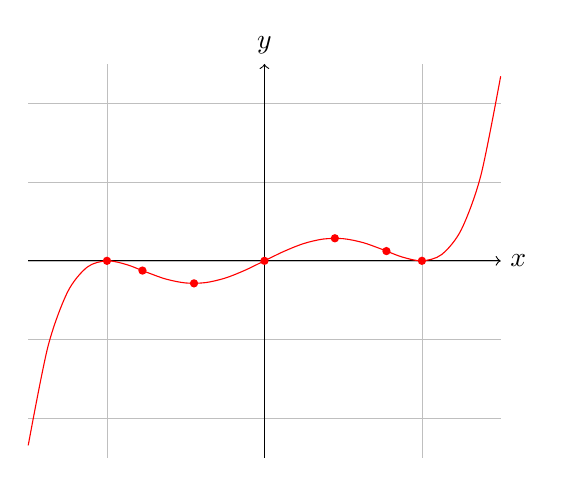
\begin{tikzpicture}[xscale=2]
          \draw[very thin,lightgray] (-1.5,-2.5) grid (1.5,2.5);
          \draw[->] (-1.5,0) -- (1.5,0) node[right]{$x$};
          \draw[->] (0,-2.5) -- (0,2.5) node[above]{$y$};
          \draw[color=red,domain=-1.5:1.5,smooth] plot (\x,{(\x)^5-2*(\x)^3+\x});
          \path
            let 
              \p{c1} = (-1,0),
              \p{c2} = ({-1/sqrt(5)},{-16/(25*sqrt(5))}),
              \p{c3} = ({1/sqrt(5)},{16/(25*sqrt(5))}),
              \p{c4} = (1,0),
              \p{i1} = ({-sqrt(3)/sqrt(5)},{-4*sqrt(3)/(25*sqrt(5))}),
              \p{i2} = (0,0),
              \p{i3} = ({sqrt(3)/sqrt(5)},{4*sqrt(3)/(25*sqrt(5))})
            in
              coordinate (c1) at (\p{c1})
              coordinate (c2) at (\p{c2})
              coordinate (c3) at (\p{c3})
              coordinate (c4) at (\p{c4})
              coordinate (i1) at (\p{i1})
              coordinate (i2) at (\p{i2})
              coordinate (i3) at (\p{i3});
          \node[fill=red,shape=circle,minimum size=3pt,inner sep=1pt] at (c1){};
          \node[fill=red,shape=circle,minimum size=3pt,inner sep=1pt] at (c2){};
          \node[fill=red,shape=circle,minimum size=3pt,inner sep=1pt] at (c3){};
          \node[fill=red,shape=circle,minimum size=3pt,inner sep=1pt] at (c4){};
          \node[fill=red,shape=circle,minimum size=3pt,inner sep=1pt] at (i1){};
          \node[fill=red,shape=circle,minimum size=3pt,inner sep=1pt] at (i2){};
          \node[fill=red,shape=circle,minimum size=3pt,inner sep=1pt] at (i3){};
        \end{tikzpicture}
        \\
        \mbox{(a) Critical and Inflection Points} 
        & 
        \mbox{(b) Points Joined by Appropriate Arcs}
      \end{array}$
      \caption{Graphs for problem~\ref{prob:5deg}}
      \label{fig:5deg}
    \end{figure}
  \item\label{prob:CubeRoot} %3b
    The derivatives are
    \begin{align*}
      B'(x) &= 3\cdot \frac{2}{3} x^{-1/3} - 1 = 2 x^{-1/3} - 1
      \\
      B''(x) &= -\frac{2}{3} x^{-4/3}
    \end{align*}
    The critical numbers are where $B'(x)$ doesn't exist (at $x=0$
    because we can't take a negative power of $0$) and where
    $B'(x)=0$:
    \begin{align*}
      B'(x) = 0 \implies 2x^{-1/3}-1 = 0 \implies x^{-1/3} =
      \frac{1}{2}
      \implies x^{1/3} = 2 \implies x = 2^3 = 8
    \end{align*}
    So the list of critical numbers is $c=0$, $c=8$.  With those
    critical numbers as boundaries, we obtain the following table:
    \begin{table}[htbp]
      \centering
      \begin{tabular}{|c|c|c|}
        \hline
        Interval         & $h'(x)$      & $h$
        \\
        \hline\hline
        $-\infty<x<0$    & $-$          & decreasing
        \\
        \hline
        $x=0$            & $\infty$     & stationary
        \\
        \hline
        $0<x<8$          & $+$          & decreasing
        \\
        \hline
        $x=8$            & $0$          & stationary
        \\
        \hline
        $8<x<\infty$     & $+$          & increasing
        \\
        \hline
      \end{tabular}
      \caption{Intervals of Increase/Decrease for problem~\ref{prob:CubeRoot}}
      \label{tab:CubeRootfp}
    \end{table}
  \item %3c
    The derivatives are
    \begin{align*}
      G'(x) &= 1 - 4 \cdot \frac{1}{2} x^{-1/2} = 1 - 2 x^{-1/2}
      \\
      G''(x) &= -2 \cdot -\frac{1}{2} x^{-3/2} = x^{-3/2}
    \end{align*}
  \item %3d
    The derivatives are
    \begin{align*}
      f'(t) &= 1 - \sin t
      \\
      f''(t) &= -\cos t
    \end{align*}
  \end{enumerate}
\item\label{prob:x4x-13} %7
  By the product and chain rules, the first derivative of $f$ is
  \begin{equation*}
    f'(x)=4x^3(x-1)^3+x^4\cdot 3(x-1)^2\frac{d}{dx}(x-1) = 4x^3(x-1)^3
    + 3x^4(x-1)^2
  \end{equation*}
  We will find it helpful (to answer this question and for taking the
  second derivative) to factor $f'$ by taking out the lowest power of
  each factor before we go any further:
  \begin{equation*}
    f'(x) = x^3(x-1)^2\left[4(x-1) + 3x\right] = x^3(x-1)^2(7x-4)
    = 7x^3(x-4/7)(x-1)^2
  \end{equation*}
  The critical numbers are the zeros of $f'(x)$, namely $x=0$,
  $x=4/7$, and $x=1$.  Taking the second derivative of $f$ by applying
  the product rule twice, we have
  \begin{multline*}
    f''(x) = \left(\frac{d}{dx} x^3\right) \left[(x-1)^2(7x-4)\right]
    + x^3 \frac{d}{dx} \left[(x-1)^2(7x-4)\right]
    \\
    = \left(\frac{d}{dx}\right) (x-1)^2(7x-4)
    + x^3 \left(\frac{d}{dx}(x-1)^2\right) (7x-4)
    + x^3 (x-1)^2 \left(\frac{d}{dx} (7x-4)\right)
    \\
    = 3x^2(x-1)^2(7x-4) + x^3 \cdot 2(x-1) (7x-4) + x^3(x-1)^2 \cdot 7
  \end{multline*}
  There is no need to simplify $f''$, but you can if you want by
  taking out the lowest power of each factor that appears the terms of
  the above expression:
  \begin{multline*}
    f''(x) = x^2(x-1)\left[3(x-1)(7x-4) + 2x(7x-4) + 7x(x-1)\right]
    \\
    = x^2(x-1)\left[21x^2-33x+4+14x^2-8x+7x^2-7x\right]
    = x^2(x-1) (42x^2-48x+4)
  \end{multline*}
  You might be able to factor further, but there is no need.

  Applying the second derivative test at the critical number $x=0$ we
  have $f''(0)=0$ so the test is inconclusive there.  Similarly, the
  second derivative test is inconclusive at $x=1$ because $f''(1)=0$.
  However, the second derivative test is conclusive at $x=4/7$ because
  \begin{equation*}
    f''(4/7) = (4/7)^2(4/7-1) (42(4/7)^2-48(4/7)+4) = (+)(-)(+4)(42/49 - 48/7+1)
    = (+)(-)(+)(-) \ge 0
  \end{equation*}
  so by the second derivative test $f$ has a local minimum at $x=4/7$.

  The first derivative test is better in this case.  Using the factors
  of the first derivative
  \begin{equation*}
    f'(x)= 7x^3(x-4/7)(x-1)^2
  \end{equation*}
  and the critical numbers we obtain Table~\ref{tab:x4x-13fp}.
  \begin{table}[htbp]
    \centering
    \begin{tabular}{|c|c|c|c|c|c|}
      \hline
      Interval      & $x^3$ & $x-4/7$ & $(x-1)^2$ & $f'(x)$ & $f$
      \\
      \hline\hline
      $-\infty<x<0$ & $-$   & $-$     & $+$       & $+$     & increasing
      \\
      \hline
      $x=0$         & $0$   & $-$     & $+$       & $0$     & stationary
      \\
      \hline
      $0<x<4/7$     & $+$   & $-$     & $+$       & $-$     & decreasing
      \\
      \hline
      $x=4/7$       & $+$   & $0$     & $+$       & $0$     & stationary
      \\
      \hline
      $4/7<x<1$     & $+$   & $+$     & $+$       & $+$     & increasing
      \\
      \hline
      $x=1$         & $+$   & $+$     & $0$       & $0$     & stationary
      \\
      \hline
      $1<x<\infty$  & $+$   & $+$     & $+$       & $+$     & increasing
      \\
      \hline
    \end{tabular}
    \caption{Intervals of Increase/Decrease for problem~\ref{prob:x4x-13}}
    \label{tab:x4x-13fp}
  \end{table}
  According to the table, $f(x)$ has a local maximum at the critical
  number $x=0$ (which the second derivative test didn't detect), a
  local minimum at the critical number $x=4/7$ (which agrees with the
  second derivative test) and neither a minimum nor a maximum at the
  critical number $x=1$ (where again the second derivative test was
  inconclusive).
\item\label{prob:funknown} %11
  We don't know what $f$ is, but we only need $f'$ to construct our
  usual table for intervals of increase/decrease.  The critical
  numbers are at the zeros of $f'$, namely $x=-1$, $x=3$, and $x=6$,
  which gives us Table~\ref{tab:funknown}.
  \begin{table}[htbp]
    \centering
    \begin{tabular}{|c|c|c|c|c|c|}
      \hline
      Interval       & $(x+1)^2$ & $(x-3)^5$ & $(x-6)^4$ & $f'(x)$ & $f$
      \\
      \hline\hline
      $-\infty<x<-1$ & $+$       & $-$       & $+$       & $-$     & decreasing
      \\
      \hline
      $x=-1$         & $0$       & $-$       & $+$       & $0$     & stationary
      \\
      \hline
      $-1<x<3$       & $+$       & $-$       & $+$       & $-$     & decreasing
      \\
      \hline
      $x=3$          & $+$       & $0$       & $+$       & $0$     & stationary
      \\
      \hline
      $3<x<6$        & $+$       & $+$       & $+$       & $+$     & increasing
      \\
      \hline
      $x=6$          & $+$       & $+$       & $0$       & $0$     & stationary
      \\
      \hline
      $6<x<\infty$   & $+$       & $+$       & $+$       & $+$     & increasing
      \\
      \hline
    \end{tabular}
    \caption{Intervals of Increase/Decrease for problem~\ref{prob:funknown}}
    \label{tab:funknown}
  \end{table}
  Note that the minus signs in the $(x+1)^2$ and $(x-6)^4$ columns
  have flipped to plus signs because the power is an even number in
  both cases.  We conclude that $f$ is increasing on just the
  intervals $(3,6)$ and $(6,\infty)$.
  % EJD: diagram
\item %13
  The derivatives are
  \begin{align*}
    y' &= \frac{(1+x^2)-(1+x)(2x)}{(1+x^2)^2} = (1-2x-x^2)(1+x^2)^{-2} \\
    y'' &= (-2-2x)(1+x^2)^{-2} + (1-2x-x^2)(-2)(1+x^2)^{-3}(2x)
  \end{align*}
  Simplifying the second derivative,
  \begin{align*}
    y'' &= -2(1+x^2)^{-3} \left[(x+1)(1+x^2) +(2x)(1-2x-x^2)\right]
    \\
    &= -2(1+x^2)^{-3} \left[x^3+x^2+x+1-2x^3-4x^2+2x\right]
    \\
    &= 2 (1+x^2)^{-3} (x^3+3x^2-3x-1)
  \end{align*}
  We need to further factor $y''$.  We guess roots which divide the
  constant term in the cubic $-x^3-3x^2+3x+1$, namely $1$, so our
  guesses for roots are $\pm 1$.  The root $x=1$ works so we can pull
  out a factor $(x-1)$ by polynomial division or otherwise:
  \begin{align*}
    y'' = 2(1+x^2)^{-3} (x-1)(x^2+4x+1)
  \end{align*}
  We complete factoring by using the quadratic formula to get the
  roots $x=-2-\sqrt{3}$ and $x=-2+\sqrt{3}$, so we can write
  \begin{align*}
    y'' = 2(1+x^2)^{-3} (x-(-2-\sqrt{3}))(x-(-2+\sqrt{3}))(x-1)
  \end{align*}
  The potential inflection numbers are the numbers $x$ where $y''$ is
  undefined (nowhere, since the denominator $(1+x^2)^3$ is never $0$)
  and where $y''=0$, namely $x=-2-\sqrt{3}$, $x=-2+\sqrt{3}$ and
  $x=1$.  You can make a table for the sign of $y''$ if you wish, but
  since each of the factors in the numerator is not to an even power,
  the sign of $y''$ will change across each of those potential
  inflection numbers, so the concavity will change at each of those
  potential inflection numbers, so each of those potential inflection
  numbers is an actual inflection number.  (Make a table if you are
  confused by the above discussion.)

  To find the actual inflection points, we evaluate $y$ at each of the
  inflection numbers:
  \begin{align*}
    y(-2-\sqrt{3}) = \frac{1+-2-\sqrt{3}}{1+(-2-\sqrt{3})^2}
    = \frac{-1-\sqrt{3}}{1+4+4\sqrt{3}+3}
    = \frac{-1-\sqrt{3}}{8+4\sqrt{3}}
    = -\frac{1}{4} \frac{1+\sqrt{3}}{2+\sqrt{3}}
  \end{align*}
  It will be convenient to rationalize the denominator by multiplying
  through by the conjugate of the denominator:
  \begin{equation*}
    y(-2-\sqrt{3}) 
    = -\frac{1}{4}\frac{(1+\sqrt{3})(2-\sqrt{3})}{(2+\sqrt{3})(2-\sqrt{3})}
    = -\frac{1}{4} \frac{-1+\sqrt{3}}{1}
    = \frac{1}{4} (1-\sqrt{3})
  \end{equation*}
  Similarly (just changing some of the plus signs to minus signs in
  the above two calculations) we obtain
  \begin{equation*}
    y(-2+\sqrt{3})
    = \frac{1}{4} (1+\sqrt{3})
  \end{equation*}
  and obviously $y(1)=(1+1)/(1+1)=1$.  So the three points of inflection
  are
  \begin{equation*}
    \mbox{$(-2-\sqrt{3},1/4-(1/4)\sqrt{3})$,
      $(-2+\sqrt{3},1/4+(1/4)\sqrt{3})$,
      and $(1,1)$}
  \end{equation*}
  There are various ways to show that three points lie on a straight
  line, the most straightforward of which is to find the line through
  two of the points and show that the third point lies on that line.
  We find the line through the first two inflection points.  The slope
  of the line is
  \begin{equation*}
    m = \frac{y_2-y_1}{x_2-x_1}
    = \frac{(1/4)(1+\sqrt{3})-(1/4)(1-\sqrt{3})}{(-2+\sqrt{3})-(-2-\sqrt{3})}
    = \frac{1}{4} \frac{2\sqrt{3}}{2\sqrt{3}} = \frac{1}{4}
  \end{equation*}
  So one way to write the equation of the line through the first two 
  inflection points is
  \begin{equation*}
    y-y_1 = m(x-x_1) \implies
    y-\frac{1}{4}(1-\sqrt{3}) = \frac{1}{4} (x-(-2-\sqrt{3}))
  \end{equation*}
  Obviously the second inflection point lies on that line, so we only
  need to check whether the third inflection point $(1,1)$ also lies
  on it.  The left hand side of the equation for the line is
  \begin{equation*}
    1-\frac{1}{4}(1-\sqrt{3}) = \frac{3}{4} + \frac{1}{4}\sqrt{3}
  \end{equation*}
  while the right hand side is
  \begin{equation*}
    \frac{1}{4} (1-(-2-\sqrt{3}) = \frac{1}{4} (3+\sqrt{3})
    = \frac{3}{4} + \frac{1}{4} \sqrt{3}
  \end{equation*}
  Since the LHS and the RHS agree, $(1,1)$ also lies on the line, so
  all three points lie on the same straight line.
\end{enumerate}
\end{document}

%%%%%%%%%%%%%%%%%%%%%%%%%%%%%%%%%%%%%%%%%%%%%%%%%%%%%%%%%%%%%%%%%%%%%%
%%% MATH110-PS033-Solutions.tex ends here
